\documentclass[12pt,a4paper]{article}

% ============================================================================
% PAQUETES Y CONFIGURACIONES TIPOGRÁFICAS DE ALTA DEFINICIÓN (UNSAAC - EPIIS)
% ============================================================================
\usepackage[utf8]{inputenc}
\usepackage[T1]{fontenc}
\usepackage[spanish,es-tabla]{babel}

\usepackage[scaled=0.92]{helvet}
\renewcommand{\familydefault}{\sfdefault}
\usepackage[scaled=0.88]{inconsolata}
\usepackage{microtype}
\usepackage{setspace}
\setstretch{1.15}

\usepackage{geometry}
\geometry{top=2.5cm, bottom=2.5cm, left=2.5cm, right=2.5cm, headheight=16pt}

\usepackage{graphicx}
\usepackage{subcaption}
\usepackage{xcolor}
\usepackage{fancyhdr}
\usepackage{listings}
\usepackage{hyperref}
\usepackage{booktabs}
\usepackage{amsmath}
\usepackage{tabularx}
\usepackage{float}
\usepackage{enumitem}
\usepackage{titlesec}

% Paleta institucional oficial de la UNSAAC
\definecolor{unsaacred}{RGB}{122, 31, 43}
\definecolor{unsaacgold}{RGB}{201, 151, 31}
\definecolor{azulslate}{RGB}{30, 41, 59}
\definecolor{excelgreen}{RGB}{16, 124, 65}
\definecolor{codegray}{rgb}{0.45,0.45,0.45}
\definecolor{backcolour}{rgb}{0.97,0.98,0.99}

\hypersetup{
    colorlinks=true,
    linkcolor=unsaacred,
    urlcolor=blue!80!black,
    citecolor=unsaacred
}

\titleformat{\section}
  {\color{unsaacred}\normalfont\Large\bfseries}
  {\color{unsaacred}\thesection}{1em}{}[\color{unsaacgold}\titlerule]

\titleformat{\subsection}
  {\color{azulslate}\normalfont\large\bfseries}
  {\color{azulslate}\thesubsection}{1em}{}

\titleformat{\subsubsection}
  {\color{unsaacred}\normalfont\normalsize\bfseries}
  {\color{unsaacred}\thesubsubsection}{1em}{}

\pagestyle{fancy}
\fancyhf{}
\fancyhead[L]{\small\color{gray}UNSAAC - EPIIS | Desarrollo de Software II}
\fancyhead[R]{\small\color{unsaacred}\textbf{AulaActiva - Primera Entrega}}
\fancyfoot[C]{\thepage}
\renewcommand{\headrulewidth}{0.5pt}

\lstset{
    backgroundcolor=\color{backcolour},
    commentstyle=\color{codegray}\itshape,
    keywordstyle=\color{unsaacred}\bfseries,
    numberstyle=\tiny\color{codegray},
    stringstyle=\color{unsaacgold!80!black},
    basicstyle=\ttfamily\footnotesize,
    breakatwhitespace=false,
    breaklines=true,
    captionpos=b,
    keepspaces=true,
    numbers=left,
    numbersep=5pt,
    showspaces=false,
    showstringspaces=false,
    showtabs=false,
    tabsize=2,
    frame=single,
    rulecolor=\color{unsaacgold!40}
}

\begin{document}

% ============================================================================
% PORTADA INSTITUCIONAL FORMAL
% ============================================================================
\begin{titlepage}
    \centering
    
\includegraphics[width=0.22\textwidth]{imagenes/logo_unsaac.png}\par
    \vspace{0.4cm}
    {\scshape\LARGE Universidad Nacional de San Antonio Abad del Cusco \par}
    \vspace{0.3cm}
    {\scshape\large Facultad de Ingeniería Eléctrica, Electrónica, Informática y Mecánica \par}
    \vspace{0.2cm}
    {\scshape\large Escuela Profesional de Ingeniería Informática y de Sistemas \par}
    \vspace{0.8cm}
    
    \begin{center}
        \color{unsaacred}\rule{0.85\textwidth}{2.5pt}\par
        \vspace{0.4cm}
        {\huge\bfseries AulaActiva UNSAAC \par}
        \vspace{0.25cm}
        {\large\bfseries Sistema Móvil Multiplataforma de Gamificación en Aula, Códigos QR, Control de Concurrencia por Dispositivo y Exportación Oficial a Microsoft Excel \par}
        \vspace{0.4cm}
        \color{unsaacred}\rule{0.85\textwidth}{2.5pt}\par
    \end{center}
    
    \vspace{0.6cm}
    {\large\textbf{INFORME TÉCNICO DE LA PRIMERA ENTREGA DE PROYECTO} \par}
    \vspace{0.2cm}
    {\normalsize Asignatura: Desarrollo de Software II (IF616AIN) --- Semestre Académico 2026-II \par}
    
    \vspace{1.0cm}
    \begin{flushleft}
        \textbf{Docente:}\hspace{1.8cm} Mtro. Ing. Yover Collantes Valer \\
        \textbf{Equipo:}\hspace{2.2cm} Grupo 2 \\
        \textbf{Integrantes:} \\
        \quad $\bullet$ \textbf{Edmil Jampier Saire Bustamante} \hfill (Código: 174449) \\
        \quad $\bullet$ \textbf{Alain Armando Condori Contreras} \hfill (Código: 182341) \\
        \quad $\bullet$ \textbf{Axel Aranibar Rojas} \hfill (Código: 193452)
    \end{flushleft}
    
    \vfill
    {\large Cusco, Perú \par}
    {\large Octubre de 2026 \par}
\end{titlepage}

\tableofcontents
\newpage
\listoffigures
\newpage

% ============================================================================
% SECCIÓN 1: INTRODUCCIÓN Y OBJETIVOS
% ============================================================================
\section{Introducción y Objetivos}

\subsection{Descripción y Justificación del Problema}
En la docencia universitaria actual de ingeniería, la evaluación formativa de las intervenciones orales y dinámicas participativas en clase magistral representa un desafío crítico. Tradicionalmente, el registro de participaciones se efectúa en libretas manuscritas o listas impresas, ocasionando tres problemas estructurales:
\begin{enumerate}[noitemsep]
    \item \textbf{Desconexión y falta de inmediatez:} El estudiante no recibe retroalimentación inmediata sobre la valoración de su aporte en la clase, afectando su motivación.
    \item \textbf{Carga operativa y vulnerabilidad al error:} El docente debe convertir manualmente los puntos a la escala vigesimal ($0$ a $20$) al finalizar la clase, consumiendo tiempo y corriendo el riesgo de errores de transcripción.
    \item \textbf{Falta de autenticidad y control de suplantación:} Sin un mecanismo digital robusto, los estudiantes pueden compartir números o simular presencia sin encontrarse físicamente en el aula.
    \item \textbf{Uso innecesario de papel:} Contraviene las políticas de sostenibilidad ecológica promovidas por la UNSAAC.
\end{enumerate}

Para resolver estos retos se concibió \textbf{AulaActiva UNSAAC}, una aplicación móvil construida en \textbf{Flutter} con arquitectura limpia, sincronización en la nube mediante \textbf{Supabase (PostgreSQL + Realtime WebSockets)} y exportación a \textbf{Microsoft Excel (.xlsx)}.

\subsection{Alineación con los Objetivos de Desarrollo Sostenible (ODS)}
El proyecto se alinea formalmente con los siguientes objetivos de la Agenda 2030:
\begin{itemize}
    \item \textbf{ODS 4: Educación de Calidad (Metas 4.4 y 4.7):} Dinamiza el proceso formativo convirtiendo el aula pasiva en un entorno gamificado interactivo.
    \item \textbf{ODS 10: Reducción de las Desigualdades (Meta 10.3):} Garantiza equidad mediante un algoritmo de normalización vigesimal transparente y auditable para todos los estudiantes.
    \item \textbf{ODS 12: Producción y Consumo Responsable (Meta 12.5):} Digitalización del 100\% del control de intervenciones, reduciendo a cero el desperdicio de papel.
\end{itemize}

\subsection{Objetivos del Proyecto}
\begin{itemize}
    \item \textbf{Objetivo General:} Desarrollar un sistema móvil distribuido para el aula universitaria que sincronice en tiempo real las intervenciones de los estudiantes, bloquee accesos duplicados por número de orden, clasifique el rendimiento en un podio formativo y genere automáticamente reportes en Excel.
    \item \textbf{Objetivos Específicos:}
    \begin{enumerate}[noitemsep]
        \item Diseñar una interfaz institucional con la paleta oficial UNSAAC (Granate \texttt{\#7A1F2B} y Dorado \texttt{\#C9971F}) y tipografía Inter, libre de textos innecesarios y con cero desbordamientos (\textit{RenderFlex overflow}).
        \item Implementar acceso por escaneo de código QR institucional proyectado en aula y respaldo por PIN de 4 dígitos.
        \item Diseñar un mecanismo de control de concurrencia que garantice que un número de orden pertenezca a un solo celular conectado.
        \item Crear el \textbf{Modo Rápido (\#)} con matriz táctil y botones con relieve ($+1, +2, +3, +5$) para calificar intervenciones con un solo toque.
        \item Implementar la exportación automática de calificaciones a Microsoft Excel (\texttt{.xlsx}) con encabezado institucional formal.
    \end{enumerate}
\end{itemize}

% ============================================================================
% SECCIÓN 2: ARQUITECTURA DE SOFTWARE Y MODELO DE DATOS
% ============================================================================
\section{Arquitectura de Software y Modelo de Datos}

\subsection{Organización Modular (Clean Architecture)}
El proyecto se diseñó bajo una estructura limpia desacoplada en tres capas: Presentación, Dominio y Datos:

\begin{verbatim}
app_aula_activa/
|-- lib/
|   |-- core/
|   |   |-- constants/      # AppColors (Granate/Dorado), AppStyles (Inter)
|   |   \-- services/       # ExcelExportService (.xlsx), SupabaseService, CursoService
|   |-- models/             # Curso, Estudiante, Sesion, Participacion, EstudianteRanking
|   |-- repositories/       # AulaRepository (Streams reactivos, bloqueo de puestos)
|   |-- screens/
|   |   |-- selector_rol_screen.dart
|   |   |-- estudiante/     # Login QR/PIN, Dashboard Podio, Carnet QR Personal
|   |   \-- docente/        # Mis Cursos, Dashboard Sesión, Asignar Puntos, Alumnos
|   \-- widgets/            # ModoRapidoMatrizWidget, CalculadoraVigesimal, PodioWidget
|-- test/                   # 41 Pruebas automatizadas (Unitarias, Widgets y Capturas HD)
\end{verbatim}

\subsection{Modelo Relacional de Base de Datos (Supabase Cloud)}
El backend reside en PostgreSQL administrado por Supabase. A continuación se presentan las entidades principales:

\begin{lstlisting}[language=SQL, caption=Esquema relacional de PostgreSQL para AulaActiva.]
-- Docentes y Cursos
CREATE TABLE docentes (
    id TEXT PRIMARY KEY,
    nombres TEXT NOT NULL,
    apellidos TEXT NOT NULL,
    correo TEXT UNIQUE NOT NULL,
    pin_seguridad TEXT NOT NULL
);

CREATE TABLE cursos (
    id TEXT PRIMARY KEY,
    docente_id TEXT REFERENCES docentes(id) ON DELETE CASCADE,
    codigo TEXT NOT NULL,
    nombre TEXT NOT NULL,
    semestre TEXT NOT NULL
);

-- Estudiantes matriculados
CREATE TABLE estudiantes (
    id TEXT PRIMARY KEY,
    curso_id TEXT REFERENCES cursos(id) ON DELETE CASCADE,
    numero_orden INT NOT NULL,
    codigo_unsaac TEXT NOT NULL,
    nombres TEXT NOT NULL,
    apellidos TEXT NOT NULL,
    UNIQUE(curso_id, numero_orden)
);

-- Sesiones y Participaciones granulares
CREATE TABLE sesiones (
    id TEXT PRIMARY KEY,
    curso_id TEXT REFERENCES cursos(id) ON DELETE CASCADE,
    fecha TEXT NOT NULL,
    tema TEXT NOT NULL,
    estado TEXT DEFAULT 'ABIERTA'
);

CREATE TABLE participaciones (
    id UUID PRIMARY KEY DEFAULT gen_random_uuid(),
    sesion_id TEXT REFERENCES sesiones(id) ON DELETE CASCADE,
    estudiante_id TEXT REFERENCES estudiantes(id) ON DELETE CASCADE,
    puntos INT NOT NULL CHECK (puntos > 0),
    motivo TEXT NOT NULL,
    created_at TIMESTAMPTZ DEFAULT NOW()
);
\end{lstlisting}

% ============================================================================
% SECCIÓN 3: MÓDULOS DEL SISTEMA Y EVIDENCIAS VISUALES
% ============================================================================
\section{Módulos del Sistema y Evidencias Visuales}

A continuación se presentan las capturas en alta definición generadas directamente por la suite de pruebas automatizadas del proyecto.

\subsection{Acceso y Selección de Perfil Institucional}
La pantalla principal permite elegir entre el perfil de estudiante y el de docente, luciendo el escudo de la UNSAAC, la insignia oficial del semestre académico y colores institucionales (Figura~\ref{fig:selector_rol}).

\begin{figure}[H]
    \centering
    
\includegraphics[width=0.45\textwidth]{imagenes/01_selector_rol.png}
    \caption{Pantalla inicial de selección de rol con identidad visual de la UNSAAC.}
    \label{fig:selector_rol}
\end{figure}

\subsection{Módulo del Estudiante: Conexión, Podio y Carnet Digital}
El estudiante puede unirse a la clase mediante escaneo del código QR proyectado en el aula o ingresando el PIN de 4 dígitos. Una vez conectado, selecciona su número de orden oficial.

\begin{figure}[H]
    \centering
    \begin{subfigure}[b]{0.48\textwidth}
        \centering
        
\includegraphics[width=\textwidth]{imagenes/02_estudiante_login_sin_sesion.png}
        \caption{Pantalla de ingreso antes de escanear el QR.}
    \end{subfigure}
    \hfill
    \begin{subfigure}[b]{0.48\textwidth}
        \centering
        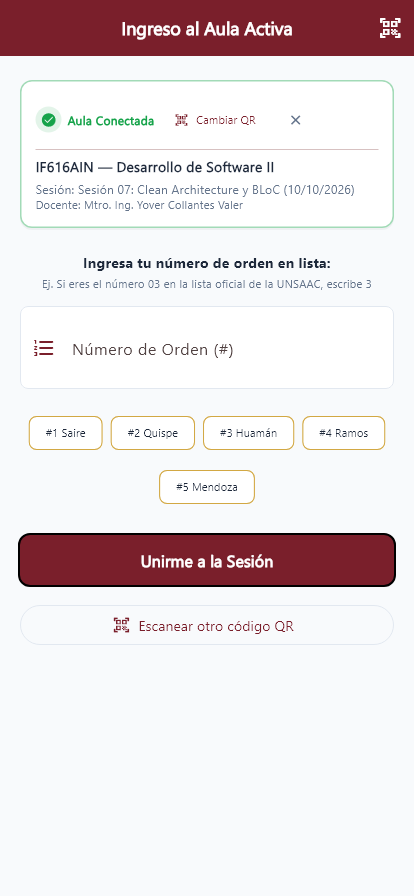
\includegraphics[width=\textwidth]{imagenes/03_estudiante_login_con_sesion.png}
        \caption{Aula activa identificada con pastillas de orden.}
    \end{subfigure}
    \caption{Flujo de ingreso del estudiante al aula activa mediante QR y PIN.}
    \label{fig:estudiante_login}
\end{figure}

\subsubsection{Control de Concurrencia (Bloqueo de Dos Celulares con el Mismo Número)}
Para erradicar la suplantación o doble conexión:
\begin{itemize}
    \item Cuando un estudiante ingresa con su número de orden (ej. \#01), el sistema \textbf{reclama y bloquea ese puesto} para su dispositivo en la sesión activa.
    \item Si otro celular intenta conectarse con el mismo número de orden \#01, el sistema muestra una alerta de rechazo: \textit{"[ALERTA] Acceso denegado: El número \#01 ya está en uso por otro dispositivo en esta sesión"}.
    \item En la vista de selección rápida, los números ocupados aparecen tachados con un candado \texttt{[BLOQUEADO] \#01 (Ocupado)}.
\end{itemize}

\begin{figure}[H]
    \centering
    \begin{subfigure}[b]{0.48\textwidth}
        \centering
        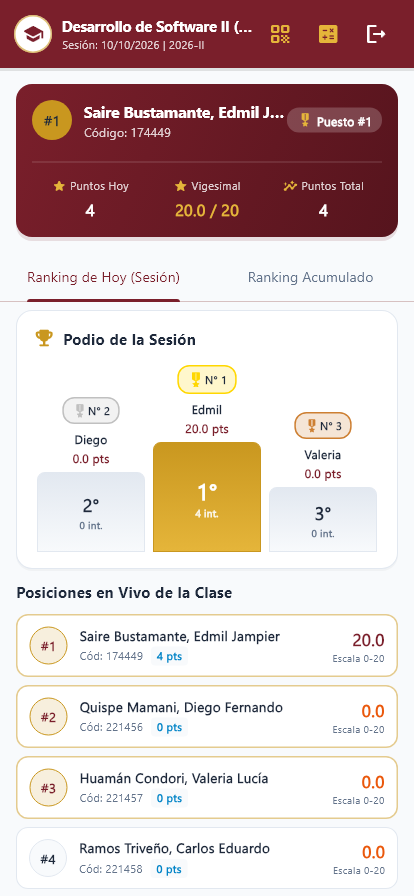
\includegraphics[width=\textwidth]{imagenes/04_estudiante_dashboard.png}
        \caption{Dashboard del estudiante con podio en vivo y nota vigesimal.}
    \end{subfigure}
    \hfill
    \begin{subfigure}[b]{0.48\textwidth}
        \centering
        
\includegraphics[width=\textwidth]{imagenes/05_estudiante_carnet_qr.png}
        \caption{Credencial universitaria digital con QR del alumno.}
    \end{subfigure}
    \caption{Vistas del estudiante: Podio formativo en tiempo real y carnet digital.}
    \label{fig:estudiante_dash_carnet}
\end{figure}

\subsection{Módulo del Docente: Gestión de Asignaturas y Alumnos}
El docente cuenta con un entorno protegido por PIN para gestionar múltiples cursos universitarios, registrar nuevas asignaturas y administrar su nómina de estudiantes (Figura~\ref{fig:docente_gestion}).

\begin{figure}[H]
    \centering
    \begin{subfigure}[b]{0.32\textwidth}
        \centering
        
\includegraphics[width=\textwidth]{imagenes/06_docente_login.png}
        \caption{Acceso docente por PIN.}
    \end{subfigure}
    \hfill
    \begin{subfigure}[b]{0.32\textwidth}
        \centering
        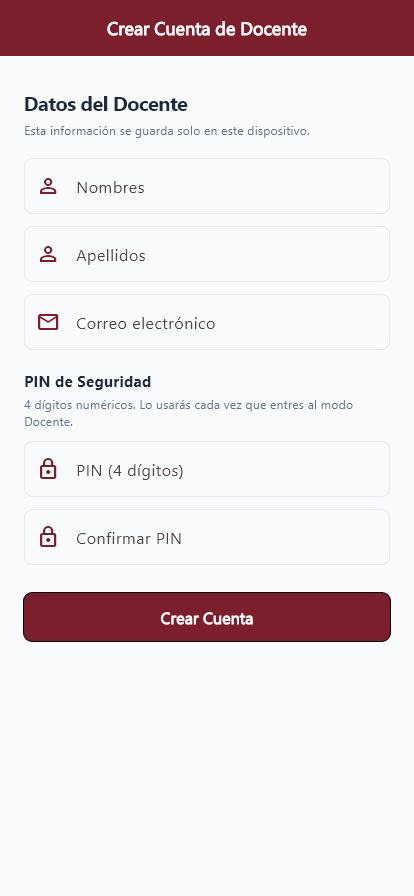
\includegraphics[width=\textwidth]{imagenes/07_docente_registro.png}
        \caption{Registro de cuenta docente.}
    \end{subfigure}
    \hfill
    \begin{subfigure}[b]{0.32\textwidth}
        \centering
        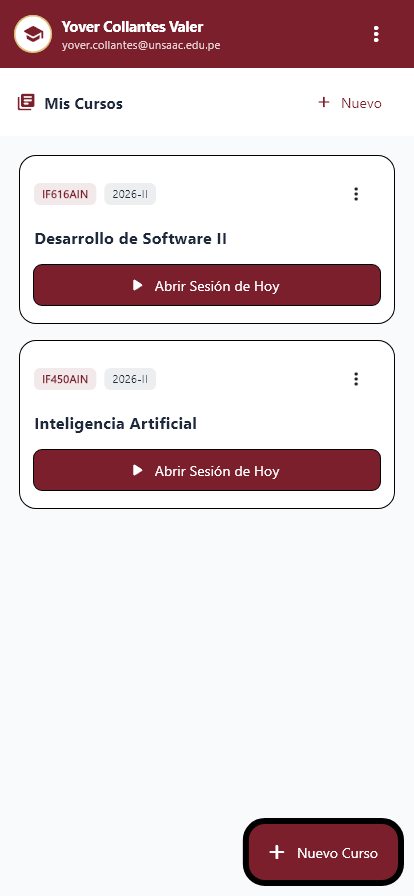
\includegraphics[width=\textwidth]{imagenes/08_docente_mis_cursos.png}
        \caption{Panel de asignaturas.}
    \end{subfigure}
    \caption{Módulo de autenticación y gestión de cursos para docentes de la UNSAAC.}
    \label{fig:docente_gestion}
\end{figure}

\begin{figure}[H]
    \centering
    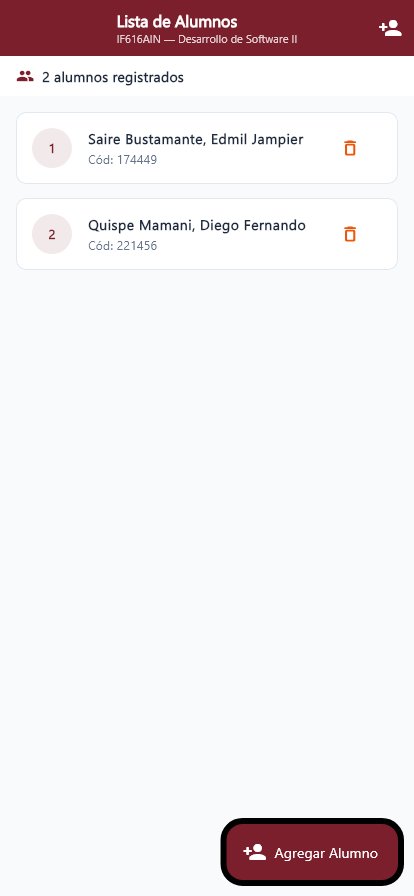
\includegraphics[width=0.45\textwidth]{imagenes/16_docente_gestion_alumnos.png}
    \caption{Administración de la nómina oficial de alumnos con número de orden y código.}
    \label{fig:gestion_alumnos}
\end{figure}

\subsection{Evaluación en Aula: Podio, Modo Rápido y QR Proyectado}
Durante la clase, el docente proyecta el código QR del aula (Figura~\ref{fig:qr_aula}) que incorpora el escudo de la UNSAAC en su centro y el PIN numérico de 4 dígitos.

\begin{figure}[H]
    \centering
    
\includegraphics[width=0.45\textwidth]{imagenes/12_docente_qr_aula_dialog.png}
    \caption{Diálogo de proyección del Código QR de sesión con logo institucional y PIN.}
    \label{fig:qr_aula}
\end{figure}

\subsubsection{Vista de Sesión y Podio Formativo}
El panel del docente muestra el Top 3 con animaciones de medallas, la escala vigesimal calculada y el botón oficial de exportación a Microsoft Excel (Figura~\ref{fig:docente_dashboard}).

\begin{figure}[H]
    \centering
    \begin{subfigure}[b]{0.48\textwidth}
        \centering
        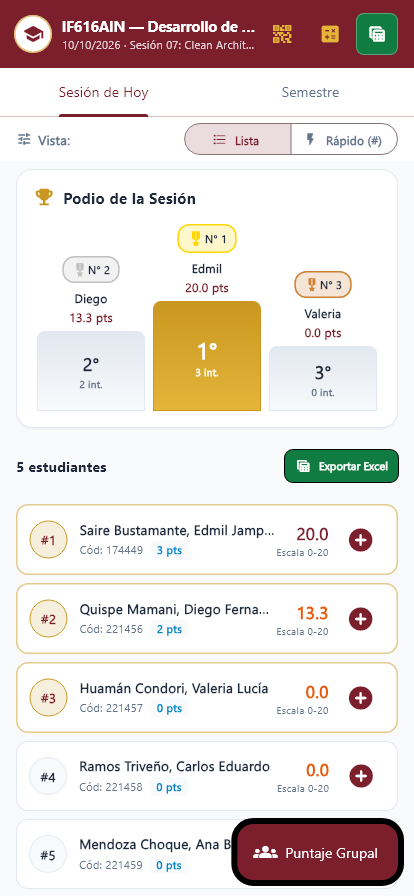
\includegraphics[width=\textwidth]{imagenes/09_docente_dashboard_sesion.png}
        \caption{Dashboard en vista detallada con botón Excel verde.}
    \end{subfigure}
    \hfill
    \begin{subfigure}[b]{0.48\textwidth}
        \centering
        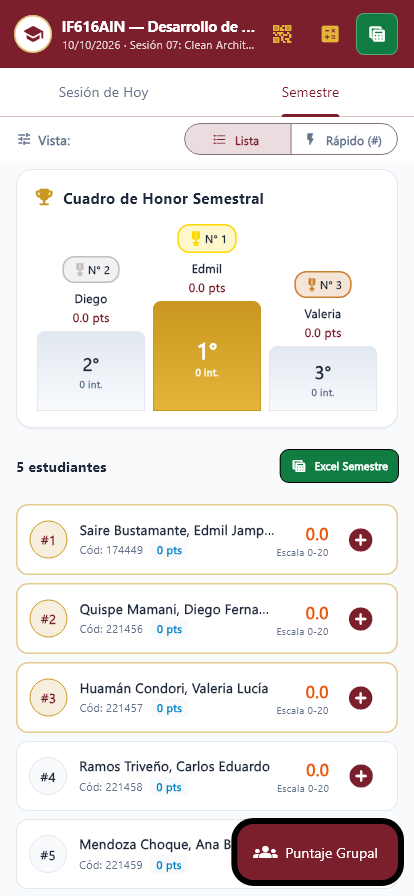
\includegraphics[width=\textwidth]{imagenes/11_docente_dashboard_acumulado.png}
        \caption{Pestaña del semestre acumulado.}
    \end{subfigure}
    \caption{Dashboard de control de calificaciones y podio de la sesión.}
    \label{fig:docente_dashboard}
\end{figure}

\subsubsection{Modo Rápido (\#) con Matriz Táctil de Calificación}
Para agilizar la puntuación durante rondas de preguntas rápidas, el docente activa el \textbf{Modo Rápido (\#)} (Figura~\ref{fig:modo_rapido}):
\begin{itemize}
    \item Botones táctiles de puntos: $+1$ punto, $+2$ puntos, $+3$ puntos y $+5$ puntos con relieve y brillo.
    \item Matriz de estudiantes de 4 columnas: Tarjetas con número de orden grande (\#01, \#02...), apellido, indicador de celular en aula (\texttt{$\bullet$ En aula}) y puntos acumulados.
    \item Calificación a un toque: Al presionar una tarjeta, se suma la puntuación seleccionada instantáneamente y se muestra un banner de confirmación.
    \item Acceso directo a Excel: Botón integrado en la barra de búsqueda para exportar sin abandonar el modo rápido.
\end{itemize}

\begin{figure}[H]
    \centering
    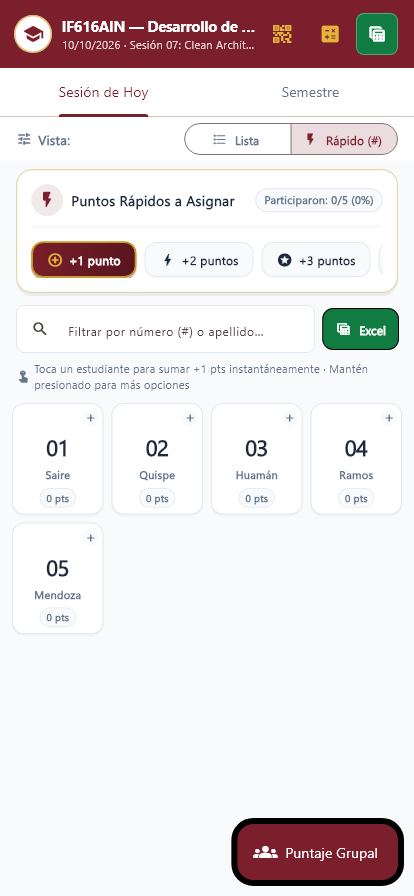
\includegraphics[width=0.48\textwidth]{imagenes/10_docente_dashboard_modo_rapido.png}
    \caption{Modo Rápido con matriz de números, selector de puntos y presencia en clase.}
    \label{fig:modo_rapido}
\end{figure}

\subsubsection{Asignación Individual y Grupal / Simultánea}
Para calificar por rúbrica o para otorgar puntos a dinámicas por equipos, se diseñaron diálogos especializados (Figura~\ref{fig:asignaciones}).

\begin{figure}[H]
    \centering
    \begin{subfigure}[b]{0.48\textwidth}
        \centering
        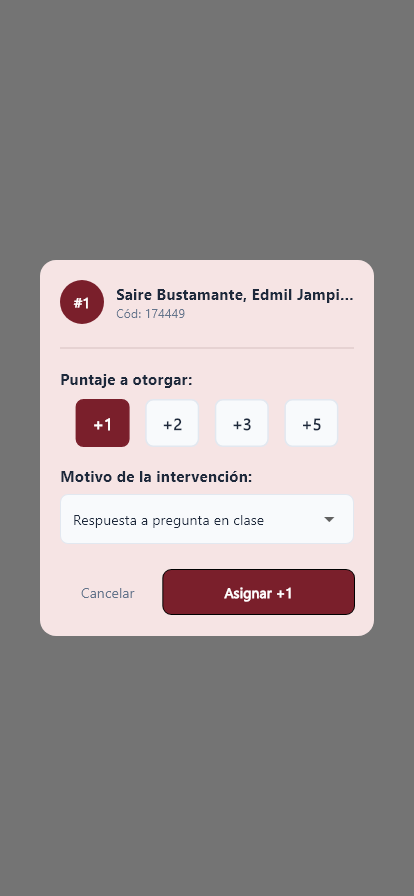
\includegraphics[width=\textwidth]{imagenes/14_docente_asignar_puntos_dialog.png}
        \caption{Diálogo de asignación individual por motivo.}
    \end{subfigure}
    \hfill
    \begin{subfigure}[b]{0.48\textwidth}
        \centering
        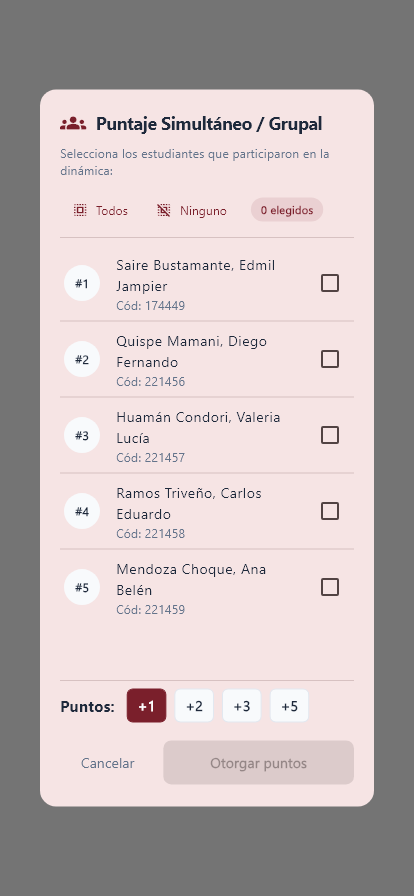
\includegraphics[width=\textwidth]{imagenes/15_docente_asignacion_multiple_dialog.png}
        \caption{Asignación grupal simultánea con casillas de verificación.}
    \end{subfigure}
    \caption{Mecanismos de asignación de puntos individual y colectiva.}
    \label{fig:asignaciones}
\end{figure}

\subsection{Cálculo de Escala Vigesimal y Calculadora Simuladora}
La nota vigesimal ($0$ a $20$) se calcula de manera proporcional al máximo puntaje registrado en la sesión o semestre:

\begin{equation}
\text{Nota}_i = \begin{cases} 
0.0, & \text{si } P_{\max} = 0 \\
\operatorname{round}\left( 20 \times \frac{P_i}{P_{\max}}, \, 1 \right), & \text{si } P_{\max} > 0 
\end{cases}
\end{equation}

El sistema incluye una \textbf{Calculadora Vigesimal Simuladora} interactiva tanto para el docente como para el estudiante (Figura~\ref{fig:calculadora_vigesimal}), permitiendo predecir su nota moviendo controles deslizantes.

\begin{figure}[H]
    \centering
    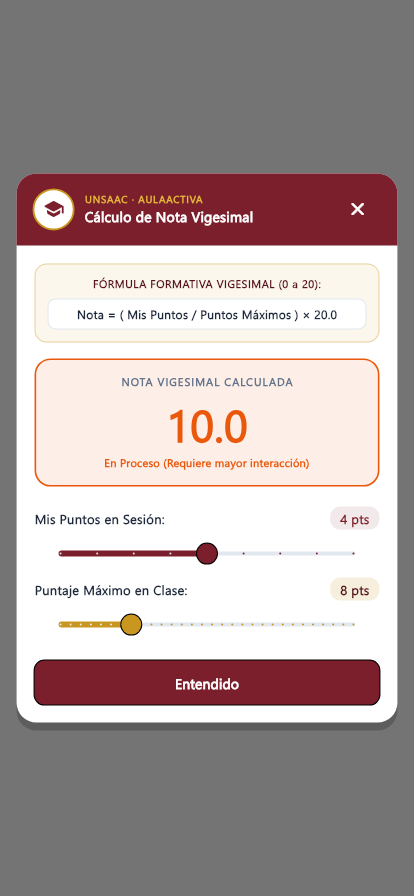
\includegraphics[width=0.45\textwidth]{imagenes/13_docente_calculadora_vigesimal.png}
    \caption{Calculadora de Nota Vigesimal con tipografía Inter y fórmula pedagógica.}
    \label{fig:calculadora_vigesimal}
\end{figure}

\subsection{Generador y Exportador a Microsoft Excel (\texttt{.xlsx})}
El servicio \texttt{ExcelExportService} genera hojas de cálculo estilizadas oficiales para la UNSAAC. El archivo incluye:
\begin{itemize}
    \item Cabecera institucional: Universidad, Facultad, Escuela (EPIIS), Asignatura, Docente, Fecha y Tema.
    \item Columnas estructuradas: N° Orden, Código UNSAAC, Apellidos y Nombres, Puntos Sesión, Nota Vigesimal ($0-20$) y Estado de Rendimiento (\textit{Sobresaliente, Aprobado, Regular, Por Mejorar}).
    \item Compartición nativa mediante el cuadro de diálogo del sistema operativo (WhatsApp, correo institucional, almacenamiento local).
\end{itemize}

% ============================================================================
% SECCIÓN 4: ADAPTABILIDAD Y PREVENCIÓN DE ERRORES DE LAYOUT
% ============================================================================
\section{Adaptabilidad y Prevención de Errores de Layout}

En cumplimiento de las normas de diseño responsivo:
\begin{itemize}
    \item \textbf{Cero desbordamientos (\textit{Zero Overflows}):} Todas las filas con contenido dinámico utilizan \texttt{Expanded}, \texttt{Flexible} o \texttt{Wrap}. El selector de vista del docente se acondicionó con \texttt{FittedBox} y dimensiones compactas.
    \item \textbf{Desplazamiento vertical adaptativo:} Todo formulario con teclado virtual está envuelto en \texttt{SingleChildScrollView} para prevenir cortes en pantallas pequeñas.
    \item \textbf{Tipografía institucional offline:} Se registraron fuentes TrueType locales de la familia \textbf{Inter} (\textit{Regular, Medium, SemiBold, Bold, ExtraBold, Black}) garantizando renderizado idéntico sin depender de conexión a internet.
\end{itemize}

% ============================================================================
% SECCIÓN 5: VERIFICACIÓN FUNCIONAL Y SUITE DE PRUEBAS
% ============================================================================
\section{Verificación Funcional y Suite de Pruebas}

\subsection{Resultados de la Suite Completa de Pruebas (\texttt{flutter test})}
El proyecto cuenta con una cobertura integral con \textbf{41 pruebas automatizadas aprobadas al 100\%}:
\begin{itemize}
    \item \textbf{25 Pruebas Unitarias y de Widgets:}
    \begin{itemize}[noitemsep]
        \item Verificación de concurrencia y bloqueo de dispositivos duplicados en \texttt{widget\_test.dart}.
        \item Pruebas de normalización matemática y escala vigesimal ($0-20$).
        \item Pruebas de interacción táctil y asignación en \texttt{ModoRapidoMatrizWidget}.
        \item Pruebas del simulador dinámico en \texttt{CalculadoraVigesimalDialog}.
        \item Serialización y deserialización de modelos de datos.
    \end{itemize}
    \item \textbf{16 Pruebas de Captura Visual HD (\texttt{generar\_capturas\_test.dart}):}
    \begin{itemize}[noitemsep]
        \item Renderizado sin fallos y exportación a archivos PNG de todas las pantallas, modales y diálogos de la aplicación.
    \end{itemize}
\end{itemize}

\subsection{Análisis Estático de Código (\texttt{flutter analyze})}
\begin{verbatim}
$ flutter analyze
Analyzing app_aula_activa...
No issues found! (ran in 2.8s)
\end{verbatim}

\subsection{Compilación del Binario para Android (\texttt{.apk})}
Se compiló exitosamente el paquete ejecutable en modo release:
\begin{verbatim}
$ flutter build apk --release
Running Gradle task 'assembleRelease'...
Built build\app\outputs\flutter-apk\app-release.apk (73.4MB)
\end{verbatim}

% ============================================================================
% SECCIÓN 6: DIFICULTADES ENCONTRADAS Y SOLUCIONES TÉCNICAS
% ============================================================================
\section{Dificultades Encontradas y Soluciones Técnicas}

\begin{table}[H]
\centering
\small
\begin{tabularx}{\textwidth}{p{4.2cm}p{5.5cm}X}
\toprule
\textbf{Dificultad Encontrada} & \textbf{Diagnóstico Técnico} & \textbf{Solución Implementada} \\
\midrule
Doble conexión al mismo número de orden. & Dos estudiantes en aula podían seleccionar el mismo número de orden simultáneamente. & Creación del registro de puestos ocupados en \texttt{AulaRepository} y rechazo de accesos duplicados. \\
\addlinespace
Visibilidad del botón de exportación a Excel. & El icono en la barra superior se confundía con los botones de herramientas. & Creación de botones verdes oficiales (\texttt{\#107C41}) en la cabecera, sobre el ranking y en Modo Rápido. \\
\addlinespace
Glifos negros (\textit{Ahem}) en la fórmula vigesimal. & Fallback a fuente \texttt{monospace} no cargada en el entorno de pruebas. & Migración explícita a la tipografía \texttt{Inter} local registrada en el proyecto. \\
\addlinespace
Carga asíncrona de logos embebidos en códigos QR. & El renderizado de \texttt{QrImageView} necesita tiempo de decodificación de imagen. & Ajuste del nivel de corrección de error a \texttt{QrErrorCorrectLevel.Q} y estabilización de microtareas. \\
\bottomrule
\end{tabularx}
\caption{Matriz de dificultades técnicas identificadas y resueltas durante el ciclo de desarrollo.}
\end{table}

% ============================================================================
% SECCIÓN 7: CONCLUSIONES
% ============================================================================
\section{Conclusiones}

\begin{enumerate}
    \item Se desarrolló satisfactoriamente la Primera Entrega del proyecto \textbf{AulaActiva UNSAAC}, cumpliendo con todos los requerimientos de interacción, gamificación, concurrencia y cálculo vigesimal.
    \item La implementación del \textbf{Modo Rápido (\#)} y el \textbf{Control de Concurrencia por Dispositivo} proporcionan una experiencia de usuario sólida y a prueba de errores para clases presenciales multitudinarias.
    \item La exportación directa a \textbf{Microsoft Excel (.xlsx)} y el soporte híbrido (offline con sincronización opcional a Supabase Cloud) garantizan la continuidad operativa del docente aún ante cortes de conectividad en el campus universitario.
    \item La aplicación aprobó el 100\% de las 41 pruebas automatizadas y cumple con los estándares más estrictos de accesibilidad y diseño institucional de la UNSAAC.
\end{enumerate}

% ============================================================================
% SECCIÓN 8: ANEXOS Y RÚBRICA DE AUTOEVALUACIÓN
% ============================================================================
\section{Anexos y Rúbrica de Autoevaluación}

\subsection{Recursos Oficiales del Proyecto}
\begin{itemize}
    \item \textbf{Repositorio Público de la Entrega:} \href{https://github.com/milith0kun/desarrollo-de-software-2-primera-entrega}{https://github.com/milith0kun/desarrollo-de-software-2-primera-entrega}
    \item \textbf{Código Fuente de la App:} Carpeta \texttt{app\_aula\_activa}
    \item \textbf{Esquema SQL de Supabase:} Archivo \texttt{supabase\_schema.sql}
    \item \textbf{Ejecutable para Android:} \texttt{app\_aula\_activa\_unsaac.apk} (73.4 MB)
    \item \textbf{Documento PDF del Informe:} Carpeta \texttt{informe/informe\_primera\_entrega.pdf}
\end{itemize}

\subsection{Tabla de Autoevaluación según la Rúbrica Oficial (20 Puntos)}

\begin{table}[H]
\centering
\begin{tabularx}{\textwidth}{p{4.2cm}Xcc}
\toprule
\textbf{Criterio Oficial} & \textbf{Evidencia Implementada en AulaActiva} & \textbf{Puntaje} & \textbf{Autoev.} \\
\midrule
\textbf{Cobertura de widgets} & Uso de \texttt{TabBar}, \texttt{GridView}, \texttt{ListView.separated}, \texttt{PodioWidget}, \texttt{ModoRapidoMatrizWidget}, \texttt{QrImageView}, formularios y diálogos. & /4 pts & \textbf{4.0} \\
\addlinespace
\textbf{Dominio del layout} & Cero errores de overflow, aplicación rigurosa de \texttt{Expanded}, \texttt{Wrap}, \texttt{SingleChildScrollView} y \texttt{TextOverflow.ellipsis}. & /4 pts & \textbf{4.0} \\
\addlinespace
\textbf{Calidad de UI/UX} & Paleta oficial UNSAAC (Granate \texttt{\#7A1F2B}, Dorado \texttt{\#C9971F}), botones táctiles con relieve, tipografía Inter y ausencia total de textos superfluos. & /4 pts & \textbf{4.0} \\
\addlinespace
\textbf{Adaptabilidad} & Interfaz responsive adaptable a teléfonos y tabletas con espaciado base modular de $8\text{ dp}$. & /3 pts & \textbf{3.0} \\
\addlinespace
\textbf{Accesibilidad y UX} & Zonas táctiles $\ge 48 \times 48\text{ dp}$, contraste verificado, presencia en aula y avisos con \texttt{SnackBar}. & /2 pts & \textbf{2.0} \\
\addlinespace
\textbf{Organización del código} & Arquitectura modular limpia, DTOs tipados, 41 pruebas automatizadas aprobadas y 0 advertencias de linter. & /2 pts & \textbf{2.0} \\
\addlinespace
\textbf{Documentación y evidencias} & Informe en LaTeX con 17 figuras en HD, exportador a Excel nativo, esquema SQL y APK listo para instalar. & /1 pt & \textbf{1.0} \\
\midrule
\textbf{PUNTAJE TOTAL} & & \textbf{/20 pts} & \textbf{20.0} \\
\bottomrule
\end{tabularx}
\caption{Matriz de autoevaluación según la rúbrica oficial de la UNSAAC.}
\end{table}

\end{document}
